\documentclass{beamer}
\usepackage{graphicx}
\usetheme{Boadilla}
\title{Area Estimation Using the Monte Carlo Method}
\subtitle{Exercise 8}
\author{Cesare De Cal}
\institute{University of Antwerp - Erasmus Exchange}
\date{December 13, 2019}
\begin{document}


% Title page
\begin{frame}
\titlepage
\end{frame}

% Problem presentation
\section{Introduction}
\subsection{Presentation}
\begin{frame}
\frametitle{The Problem}
The exercise asks to use the Monte Carlo method to approximate the area of the figure defined by
$$
\begin{cases}
1 \le x \le 3 \\
-1\le y \le 4 \\  
x^3+y^3\le 29 \\
y \ge e^x -2
\end{cases}$$
\end{frame}

\begin{frame}
\frametitle{Bounding Box}
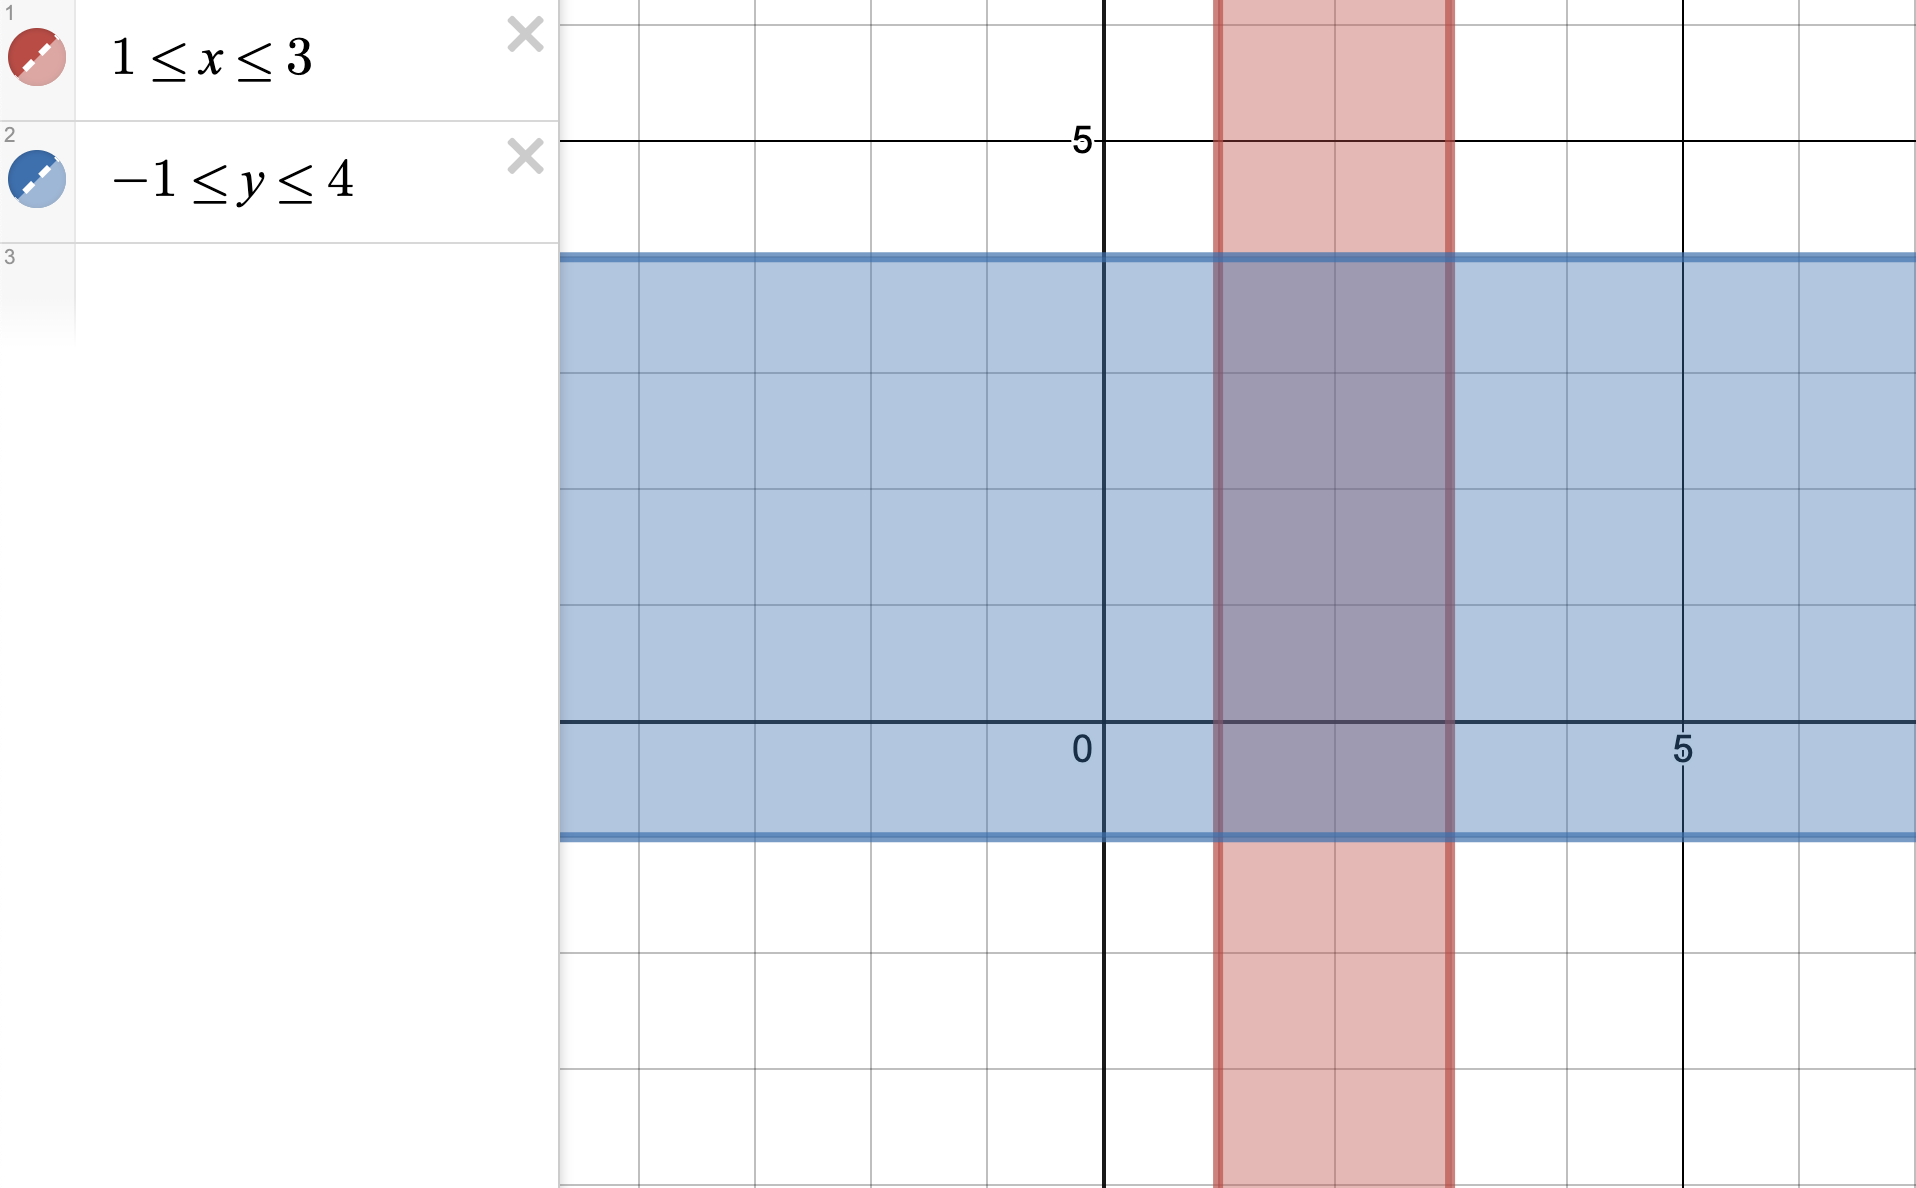
\includegraphics[width=\textwidth,height=\textheight,keepaspectratio]{bounding_box.png}
\end{frame}

\begin{frame}
\frametitle{Full System}
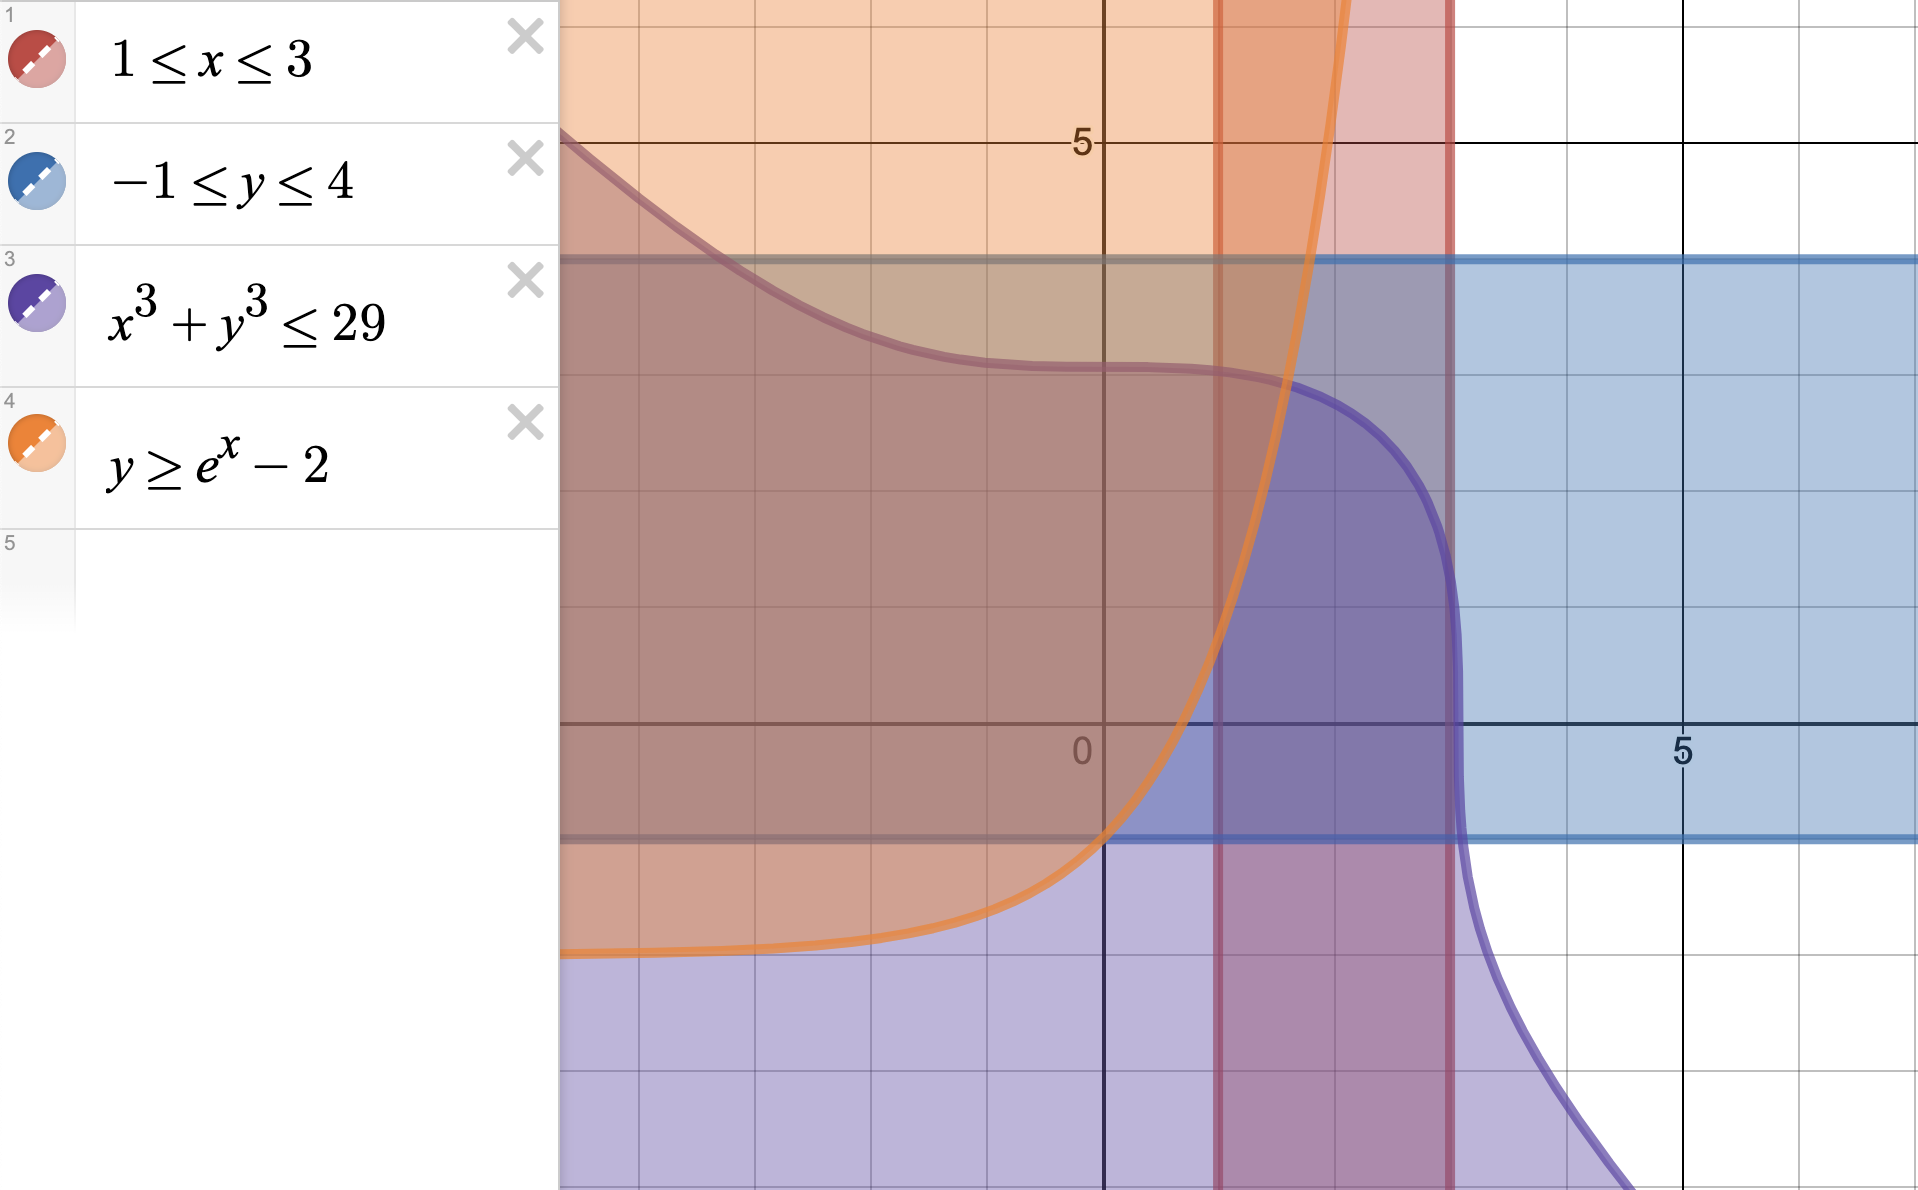
\includegraphics[width=\textwidth,height=\textheight,keepaspectratio]{full_system.png}
\end{frame}

\subsection{sub b}

\section{Section 2}

\end{document}